\section{MetaMask}\label{section:MetaMask}
Come precedentemente esposto, per utilizzare \textit{ShopChain} sarà necessario interagire con l'estensione MetaMask. Nel seguito vedremo dunque cos'è e come interagirci ai fini dell'applicativo in questione.
\subsection{Cos'è MetaMask}
MetaMask è un estensione per browser che permette di gestire wallet digitali di diverse criptovalute\glo{} che permette di effettuare transazioni sulla rete della criptovaluta in questione.
MetaMask deve essere installato nel tuo browser per tutto il tempo che userai \projectName{}, senza di esso è di fatti impossibile l'utilizzo della piattaforma.
\subsection{Installazione}
Dopo essere entrato in \projectName{}, controlla che MetaMask sia installato, puoi farlo guardando se tra le estensioni in alto a destra è presente la sua icona.
    \begin{figure}[H]
        \centering
        \includegraphics{immagini/MetaMask/MetaMask_installed.png}
        \caption{MetaMask installato correttamente}
    \end{figure}
\textbf{}\\
 Se MetaMask è installato correttamente, puoi procedere con l'utilizzo di \projectName, altrimenti procedi con l'istallazione come mostrato di seguito:\\
 Al seguente link è possibile trovare la pagina ufficiale di download di MetaMask:
 \begin{center}
     \url{https://MetaMask.io/download/}
 \end{center}
 Alla pagina sarà presente un bottone con scritto \texttt{"Install MetaMask for Chrome"}
 \begin{figure}[H]
    \centering
    \includegraphics[scale=0.3]{immagini/MetaMask/install-MetaMask.png}
    \caption{Pagina download MetaMask}
\end{figure}
\textbf{}\\
Cliccando il bottone si verrà reindirizzati alla seguente pagina web nella quale basterà cliccare il bottone \textit{"Aggiungi"}:
\begin{figure}[H]
    \centering
    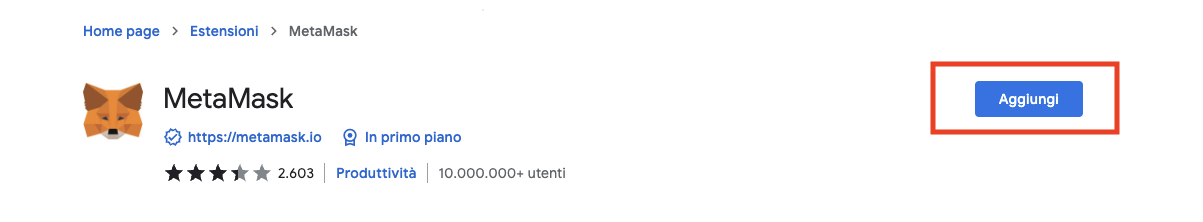
\includegraphics[scale=0.3]{immagini/MetaMAsk/MetaMaskExtensionPage.png}
    \caption{Aggiungere l'estensione MetaMask al browser (1)}
\end{figure}
\textbf{}\\
Si aprirà dunque il popup mostrato in seguito nel quale sarà sufficiente cliccare \texttt{"Aggiungi estensione"}
\begin{figure}[H]
    \centering
    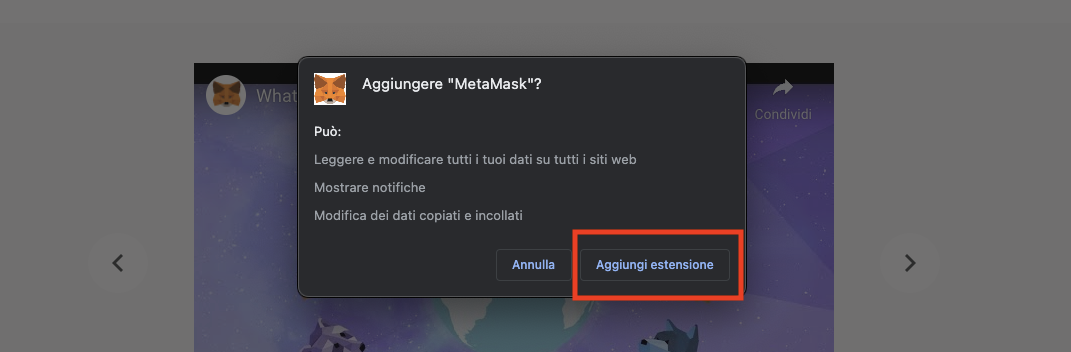
\includegraphics[scale=0.3]{immagini/MetaMAsk/AddExtenction.png}
    \caption{Aggiungere l'estensione MetaMask al browser (2)}
\end{figure}
\textbf{}\\
Una volta che l'estensione sarà stata aggiunta si verrà automaticamente reindirizzati alla pagina mostrata nella figura seguente nella quale sarà sufficiente cliccare \textit{Inizia}
\begin{figure}[H]
    \centering
    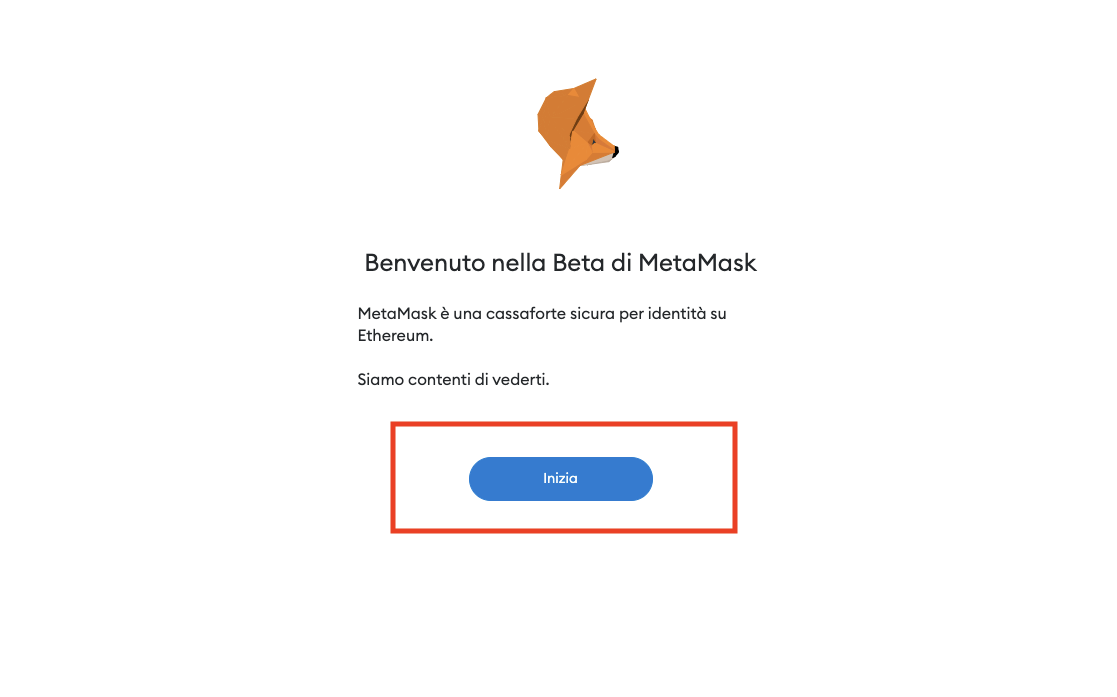
\includegraphics[scale=0.3]{immagini/MetaMask/startMetamask.png}
    \caption{Pagina iniziale MetaMask}
\end{figure}

\textbf{}\\
A questo punto non resta che scegliere se iniziare creando un nuovo portafoglio o se caricarne uno già esistente 

\begin{figure}[H]
    \centering
    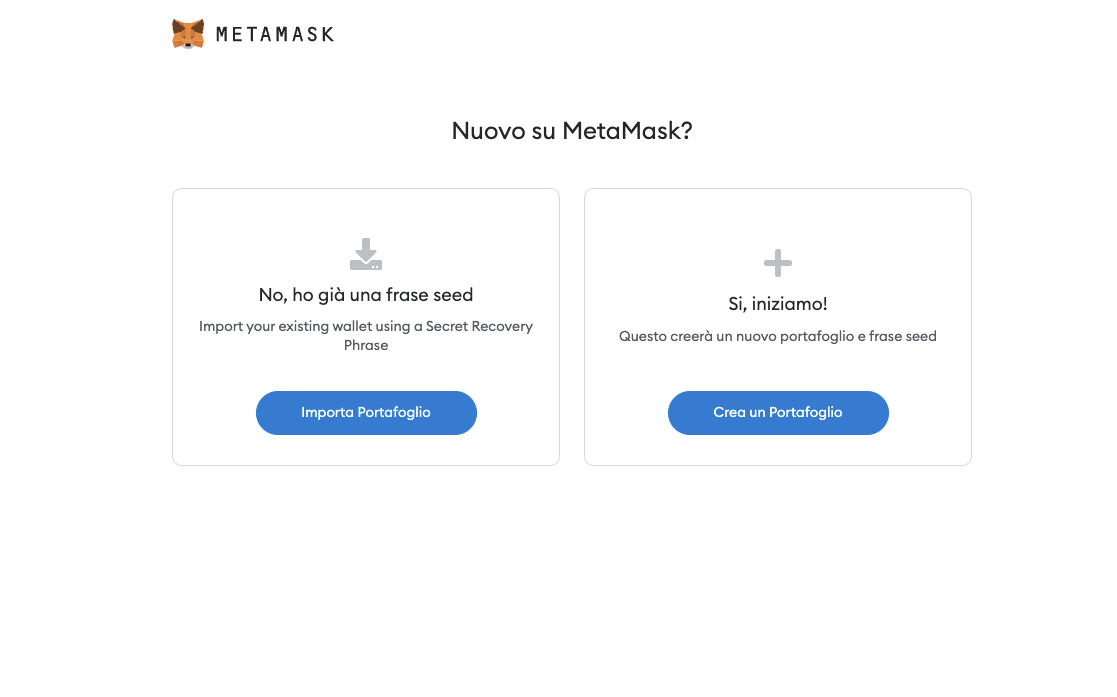
\includegraphics[scale=0.3]{immagini/MetaMask/chooseMetamask.png}
    \caption{Scelta iniziale MetaMask: crea/importa portafogli}
\end{figure}

\textbf{}\\
dopo aver scelto basterà seguire le semplici istruzioni riportate da MetaMask per completare il collegamento.

\subsection{Configurazione}
Per utilizzare l'applicazione ShopChain è necessario disporre di un account MetaMask impostato sulla testnet Fantom.
Per aggiungere una nuova rete al proprio account MetaMask, cliccare sull'estensione MetaMask, quindi su \texttt{"Rete Ethereum Principale"}  ed infine \texttt{"Aggiungi Rete"} come mostrato di seguito:
\begin{figure}[H]
    \centering
    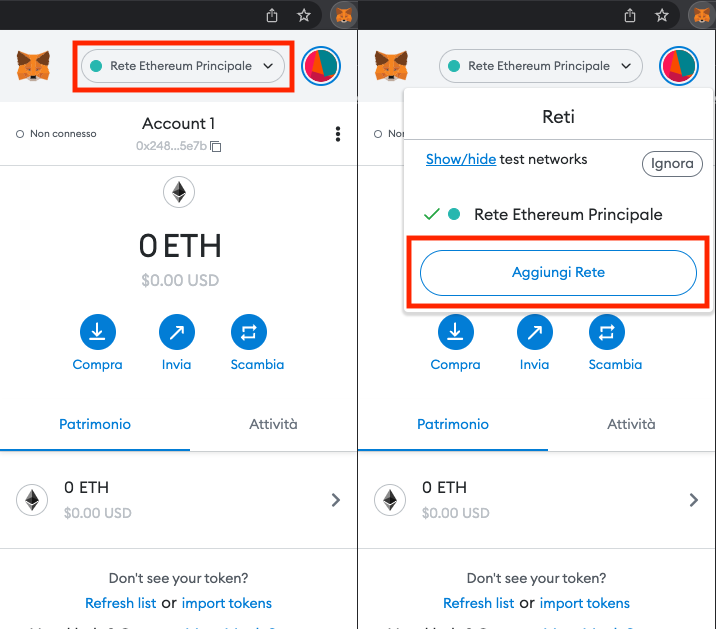
\includegraphics[scale=0.4]{immagini/MetaMask/Configuration.png}
    \caption{Inizio configurazione Fantom Testnet}
\end{figure}
\textbf{}\\
Si verrà reindirizzati ad una pagina contenente un form da riempire come mostrato di seguito:
\begin{figure}[H]
    \centering
    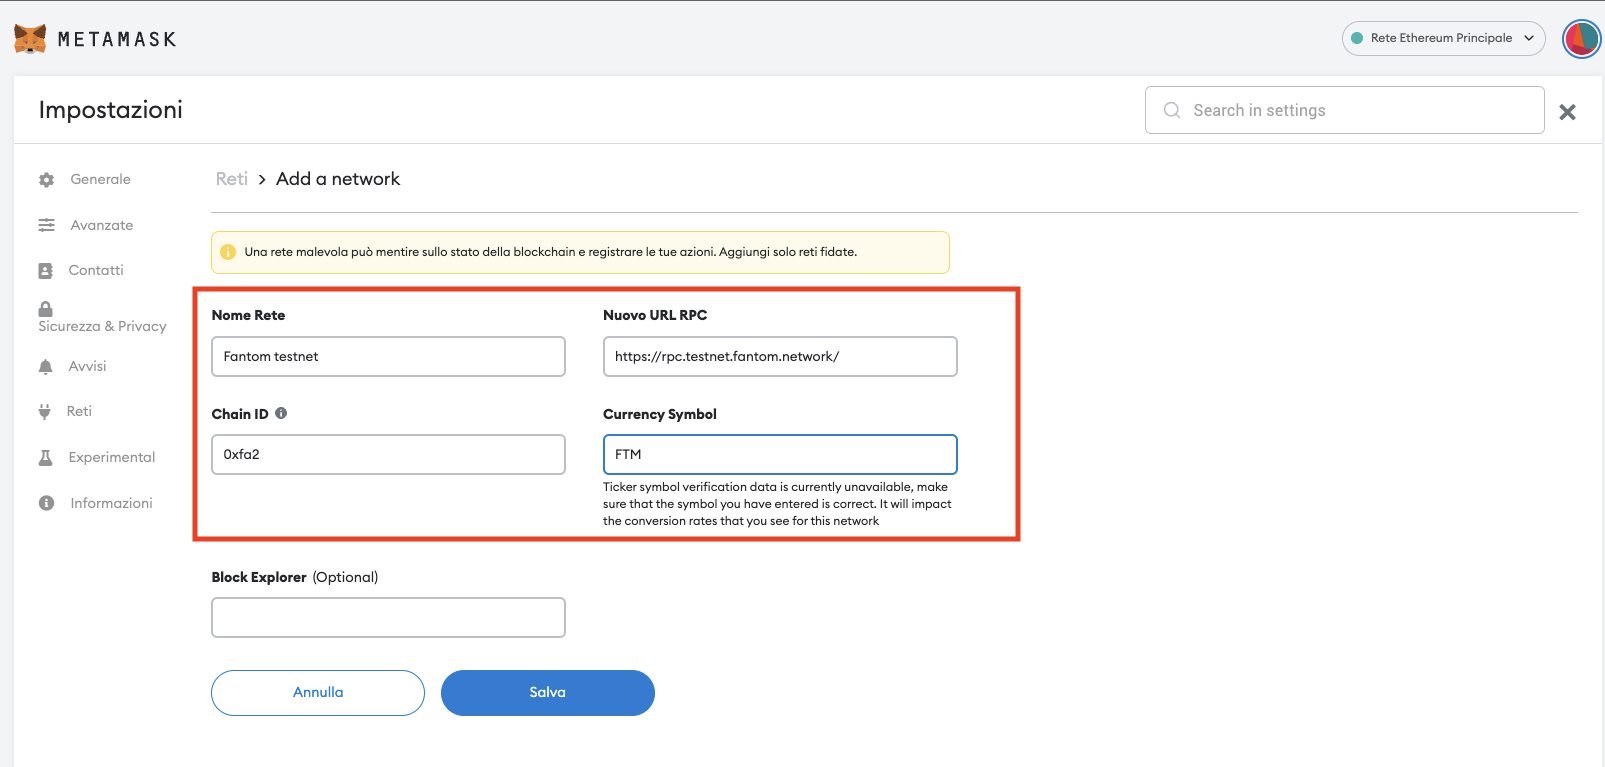
\includegraphics[scale=0.3]{immagini/MetaMask/ConfData.png}
    \caption{Form per l'aggiunta della rete Fantom Testnet}
\end{figure} 
\textbf{}\\
Per comodità vengono riportati i dati:
\begin{itemize}
    \item Network Name: Fantom testnet;
    \item New RPC Url: https://rpc.testnet.fantom.network/;
    \item ChainID: 0xfa2
    \item Symbol: FTM
\end{itemize}
Una volta riempito il form cliccare il tasto \texttt{Salva}.\\
A questo punto, una volta caricato denaro nel portafogli, sarà possibile utilizzare la piattaforma.
